\documentclass[lmodern, utf8, zavrsni]{fit}

%\batchmode
%\usepackage{booktabs}
\usepackage{listings}
\usepackage{longtable}
\usepackage{xcolor}
\usepackage{float}
\usepackage{enumitem}
\usepackage{hyperref}
\usepackage{enumerate}
\usepackage{graphicx}
\usepackage{etoolbox}
\usepackage{datetime}
\usepackage{needspace}
\usepackage{titlesec}
%\titleformat{\chapter}[display]{\normalfont\huge\bfseries}{\chaptertitlename\ \thechapter}{20pt}{\Huge}

\begin{document}
\widowpenalty=300
\clubpenalty=300

\lstset{
  language=bash,
  backgroundcolor=\color{gray!25},
  basicstyle=\ttfamily \footnotesize,
  breaklines=true,
  prebreak=\raisebox{0ex}[0ex][0ex] {\ensuremath{\hookleftarrow}},
  columns=fullflexible,
  keywords={},
  mathescape=false
}



% this alters "before" spacing (the second length argument) to 0
%\titlespacing*{\chapter}{0pt}{0pt}{40pt}

% this changes "before" spacing back to its default of 50pt
%\titlespacing*{\chapter}{0pt}{50pt}{40pt}}

%\titlespacing*{\chapter}{0pt}{-50pt}{18pt}
%\titleformat{\chapter}[display]{\normalfont\huge\bfseries}{\chaptertitlename\ \thechapter}{20pt}{\Huge}

\title{Agilni \emph{software development}\newline \color{red}{(Nacrt)}}

\author{Ernad Husremović}
\brindex{DL 2792}
\verzija {0.0.1}
\thesisnumber{00001}
\mentor{mr. Adil Joldić}

\maketitle

\tableofcontents

%\listoftables
%\listoffigures
\newpage

% abstract begin
%\begin{abstract}
%
%To be done 
%
%\keywords{open source software, OSS, Bosna i Hercegovina}
%\end{abstract}

% abstract end

\chapter{Uvod}
\vspace*{-0.7cm}

Šta znači `biti agilan'?

Agilni razvoj software-a ne predstavlja specifični proces. Agilni razvoj je način na koji se razmišlja o razvoju software-a\citep[str. 9]{agileart}.

Osnovna polazišta ovog načina razmišljanja opisuje "Agilni manifest"\footnote{\url{http://agilemanifesto.org/iso/en/principles.html}}, koji je definisan kroz četiri vrijednosti i 12 principa:

Vrijednosti:
\begin{itemize}
\item Ljudi i interakcije ispred procesa i alata
\item Software koji funkcioniše ispred iscrpne dokumentacije
\item Komunikacija sa klijentima ispred pregovora
\item Odgovor na promjene ispred slijeđenja plana
\end{itemize}

Principi:
\begin{itemize}
\item Glavni prioritet je zadovoljiti zahtjeve klijente kroz ranu i kontinuiranu \emph{isporuku} software-a
\item Blagonaklono prihvatiti \emph{promjene} funkcionalnih zahtjeva, čak i u kasnijim fazama razvoja.
\item Funkcionalan software treba isporučivati \emph{često}, nakon par hefti ili mjeseci, nastojeći da taj period bude što kraći.
\item Najefikasniji način razmejene informacija unutar razvojnog tima je direktna - `face-to-face' komunikacija.
\item Software koji \emph{funkcioniše} je primarna mjera uspjeha projekta.
\item Agilni procesi promoviraju održivi razvoj. Finansijeri, developeri i korisnici trebaju biti u stalnoj koordinaciji, bez obzira na dužinu trajanja projekta.
\item Kontinuirano pažnja na \emph{kvalitet} tehničkih operacije i dobar dizajn povećava agilnost.
\item \emph{Jednostavnost}, kao vještina postizanja maksimalnog učinka sa što manje rada, je krucijalni agilni princip.
\item Najbolja arhitektura, funkcionalni zahtjevi i dizajn se postižu u \emph{samo-organizovanim} timovima.
\item Tim redovno analizira predhodne operacije u cilju bolje efektivnosti (\emph{refleksija}). Na osnovu tih rezultata, tim podešava i koriguje buduće operacije.
\end{itemize}



\chapter{Test chapter}
\vspace*{-0.7cm}

\begin{figure}[H]
\centering
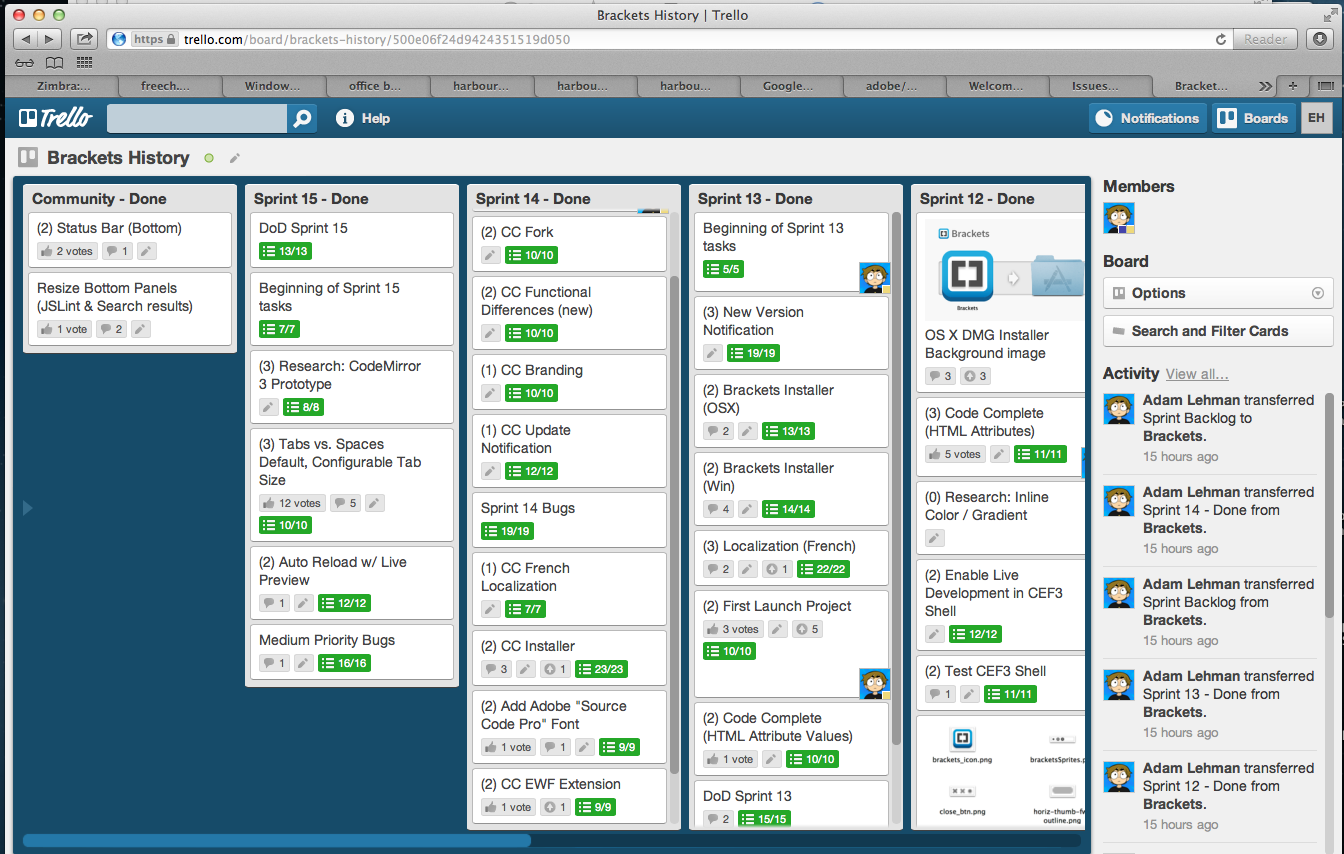
\includegraphics[width=10cm]{img/brackets_trello_sprint_history.png}
\caption{trello}
\end{figure}

\chapter{Praćenje projekta}

Defined Process Control vs Empirical Process control\citep{agiletransition}


\chapter{Zaključak}

TODO.

% -------------------------------------------------
\bibliography{literatura}
\bibliographystyle{fit}

% -------------------------------------------------
\appendix

\chapter{Instalacija}
\vspace*{-0.7cm}
\setlength{\parindent}{0cm}
%\setlength{\parindent}{default}

\chapter{Software toolset}
\begin{enumerate}
  \item Mac OS X 10.8.2
  \item mvim, vim tekst editor ver 7.3
  \item MacTex (TeX Live 2012)
\end{enumerate}

\chapter{Software repozitoriji}

\begin{itemize}
  \item Agilni developerski environment  \url{https://github.com/hernad/atile\_dev\_env}

\end{itemize}

\end{document}
